\documentclass[conference]{IEEEtran}
% SH-CADI final project report (IEEE conference format).
% Compile on Overleaf with pdfLaTeX. Figures are in ./figures/.

\usepackage{cite}
\usepackage{amsmath,amssymb}
\usepackage{graphicx}
\usepackage{booktabs}
\usepackage{array}
\usepackage{algorithm}
\usepackage{algpseudocode}
\usepackage{url}
\usepackage[hidelinks]{hyperref}

\graphicspath{{figures/}}
\renewcommand{\algorithmicrequire}{\textbf{Input:}}
\renewcommand{\algorithmicensure}{\textbf{Output:}}
\newcommand{\code}[1]{\texttt{#1}}

\begin{document}

\title{SH-CADI: A Self-Healing Content-Addressable Data Structure for Fault-Tolerant Cloud Storage Deduplication}

\author{
\IEEEauthorblockN{Dhruv Jayesh Kansagara}
\IEEEauthorblockA{CB.AI.U4AID25114}
\and
\IEEEauthorblockN{Harish Kumaar S}
\IEEEauthorblockA{CB.AI.U4AID25117}
\and
\IEEEauthorblockN{Prithve K C}
\IEEEauthorblockA{CB.AI.U4AID25122}
\and
\IEEEauthorblockN{S Sri Raghav Vatsan}
\IEEEauthorblockA{CB.AI.U4AID25151}
}

\maketitle

\begin{abstract}
Deduplicating cloud storage keeps one copy of every unique chunk and relies on a content-addressable index that maps each chunk hash to its location. Because many files share the same index records, a single corrupted record can make data unreachable for all of them, and conventional recovery replays the whole metadata journal and rebuilds the entire index even when only a few records are damaged. We present SH-CADI, a self-healing content-addressable index built from a chained hash table, a fixed-shape bucketed Merkle tree and a write-ahead journal that is sharded with the same bucket partition as the tree. SH-CADI detects corruption by comparing Merkle roots with a trusted root, localizes damaged records by top-down tree descent, recovers only those records from their journal shards, installs a candidate only if its digest matches the authenticated tree, and verifies that the trusted root is restored. Lost chunk data is recovered separately with Reed-Solomon RS(4,2) erasure coding and verified by the chunk's own SHA-256 hash. On an index of 1,000,000 records with 100 corrupted records, SH-CADI reconstructed 84 records instead of 1,000,000 and its recovery phase took 13.7~ms, compared with 14.1~s for a full rebuild and 5.39~s for a stronger targeted-repair baseline. End-to-end time, which includes an $O(n)$ detection pass common to all systems, improved by 5.7$\times$. The price is slower writes: inserts are 6.7$\times$ slower and upload throughput is 3.1$\times$ lower.
\end{abstract}

\begin{IEEEkeywords}
deduplication, content-addressable storage, Merkle tree, hash table, self-healing data structures, fault tolerance, erasure coding
\end{IEEEkeywords}

%=====================================================================
\section{Introduction}

Cloud storage holds large amounts of redundant data: the same files and blocks are uploaded repeatedly across users, versions and backups. \emph{Deduplication} removes this redundancy by splitting files into chunks, naming each chunk by a cryptographic hash of its contents, and storing each unique chunk only once~\cite{venti,datadomain}. Later copies are replaced by a reference to the existing chunk.

Deduplication concentrates risk in the \emph{index}, the data structure that maps a chunk hash to the chunk's location and reference count. After deduplication, many files depend on the same index record. A corrupted storage location, chunk reference or reference count therefore affects every file that shares the chunk. Such corruption is often silent: bit rot, hardware faults and software bugs change stored values without raising an error.

Integrity structures such as Merkle trees~\cite{merkle} can detect that the index has changed. Recovery, however, is conventionally all-or-nothing: the whole index is discarded and rebuilt from the metadata journal~\cite{venti}. The cost of this recovery grows with the size of the index $n$, not with the amount of damage $k$.

This project asks whether a deduplication index can heal itself locally, so that recovery cost follows the damage rather than the index size. We designed and implemented SH-CADI (Self-Healing Content-Addressable Data structure for deduplication Index) as a data structures and algorithms project. Its main components are a hash table for content-addressable lookup and a Merkle tree for integrity verification and fault localization, together with a recovery mechanism that supports self-healing.

The contributions of this work are:
\begin{itemize}
\item \textbf{Co-partitioned detection and recovery.} The hash-prefix bucket partition of the Merkle tree is also the shard partition of the write-ahead journal, so a damaged bucket maps to one small journal read.
\item \textbf{Verify-before-install repair.} A reconstructed record is installed only if its digest equals the digest expected by the authenticated tree; several recovery sources are tried, and records that cannot be reproduced are reported as unrecoverable rather than guessed.
\item \textbf{Read and write guards} that verify a record's bucket path in $O(s+\log B)$ and heal it before it is read or modified, so corrupted values are never written back as valid state.
\item \textbf{An evaluation} against two conventional baselines at 10,000, 100,000 and 1,000,000 records, using \emph{recovery locality} (records reconstructed divided by total records) as the main metric, together with the costs SH-CADI imposes on normal operation.
\end{itemize}

The building blocks (SHA-256 content addressing, hash tables, Merkle trees, top-down Merkle descent, write-ahead logging and Reed-Solomon coding) are existing techniques; our contribution is their composition for a deduplication index and its measured evaluation.

The rest of this report is organized as follows. Section~\ref{sec:related} reviews related work. Section~\ref{sec:design} describes the data structures, Section~\ref{sec:healing} the self-healing algorithm and Section~\ref{sec:chunks} chunk-data recovery. Section~\ref{sec:impl} covers the implementation and Section~\ref{sec:eval} the evaluation. Section~\ref{sec:discussion} discusses limitations, and Section~\ref{sec:conclusion} concludes.

%=====================================================================
\section{Related Work}
\label{sec:related}

\textbf{Deduplication systems.} Venti~\cite{venti} addresses archival blocks by the hash of their contents and coalesces duplicate blocks; its tools check an index and rebuild it from scratch, which is the conventional recovery we compare against. The Data Domain file system~\cite{datadomain} focuses on deduplication throughput with a summary vector and locality-preserving caching of the fingerprint index. Lee and Seo~\cite{leeseo} study secure deduplication with dynamic ownership management, Hamandawana \emph{et al.}~\cite{speeddedup} reduce overhead in scale-out deduplication, Xia \emph{et al.}~\cite{mean} realize deduplication storage at the unreliable edge, and Ng \emph{et al.}~\cite{livededup} deduplicate virtual machine images in an open-source cloud. These works target efficiency, security or reliability of the stored data; none of them, to our knowledge, localizes and repairs corruption in the deduplication index itself.

\textbf{Merkle trees and localization.} Merkle trees~\cite{merkle} summarize a data set in one root hash. Dynamo~\cite{dynamo} uses Merkle trees over key ranges to find out-of-sync keys between replicas by comparing roots and descending only into differing subtrees. SH-CADI applies the same top-down descent between the live index and a trusted root, then recovers the localized records from a co-partitioned journal.

\textbf{Erasure coding.} Reed-Solomon codes~\cite{reedsolomon} split data into $k$ data and $m$ parity fragments, any $k$ of which reconstruct the original. We use RS(4,2) for chunk data; it is a standard technique and not a contribution of this work.

\textbf{Novelty statement.} Our literature check was limited (eight targeted searches). We did not find a published system that combines Merkle-localized detection with a co-partitioned journal to repair a deduplication index, but this does not establish novelty.

%=====================================================================
\section{System Design}
\label{sec:design}

\subsection{Overview}

On upload, a file is split into fixed-size chunks (4~KB by default) and each chunk is hashed with SHA-256~\cite{sha}. The hash is looked up in the index. If it is present, the chunk is a duplicate: its reference count is increased and no bytes are stored. Otherwise the chunk is written to storage and a new record is inserted. Every index change is first appended to the journal shard of the record's bucket and then applied to the record's Merkle path. Each file keeps a manifest, the ordered list of its chunk hashes, from which it is reconstructed.

Each index record holds \code{chunk\_id}, \code{storage\_location}, \code{size}, \code{ref\_count} and \code{referenced\_by}. The \emph{record digest} is the SHA-256 of the first four fields together with the chunk hash; it is what the Merkle tree protects. The unbounded bookkeeping list \code{referenced\_by} is excluded from the digest.

Cloud storage is simulated with local directories: one file per chunk for plain storage, and one directory per storage node for erasure-coded storage.

\subsection{Hash Table}

The index is a separately chained hash table. The bucket index is the first 32 bits of the SHA-256 key modulo the capacity; because SHA-256 output is uniformly distributed, no further hashing is needed. The table starts with 1,024 buckets and doubles when the load factor exceeds 0.75. Insert, search, update and delete take $O(1)$ time on average and $O(n)$ in the worst case; resizing is amortized $O(1)$ per insert.

\subsection{Bucketed Merkle Tree}

The mid-review prototype built a Merkle tree over record digests sorted by hash. Each insert shifted later leaves and forced an $O(n)$ rebuild, an odd node was paired with itself, and locating a changed record needed a full $O(n)$ scan. We kept that tree unchanged as part of the conventional baseline and designed a different tree for SH-CADI.

The SH-CADI tree is a perfect binary tree with $B = 2^d$ leaves. Each leaf is a \emph{bucket} that holds the records whose hashes share the same top $d$ bits, so a record's position is fixed by its hash and never moves. A leaf is the SHA-256 of the prefix \code{bucket:} followed by the bucket's record digests in sorted order; an internal node is the SHA-256 of the prefix \code{node:} followed by its two children. The prefixes separate the two kinds of node. The depth is the smallest $d$ for which buckets hold at most four records on average, giving 4,096, 32,768 and 262,144 buckets for 10,000, 100,000 and 1,000,000 records.

\textbf{Trust model.} Only the root value \code{trusted\_root} is trusted; in a deployed system it would be signed or stored separately. The stored leaves, internal nodes and per-record digests are caches that may themselves be corrupted.

\textbf{Fail-stop updates.} Before an upsert, the bucket's stored path is recomputed with its siblings and compared with the trusted root in $O(\log B)$. If they disagree, the write is refused, so a damaged tree can never become the new trusted state. A successful upsert changes one record and recomputes one leaf-to-root path in $O(s \log s + \log B)$, where $s$ is the number of records in the bucket ($O(1)$ expected).

\subsection{Sharded Write-Ahead Journal}

The recovery information is an append-only journal with one shard per Merkle bucket, using the same bucket function as the tree. Each line stores a sequence number, the chunk hash, the operation (put or delete), the record and a checksum (the first 64 bits of SHA-256 over the line). A damaged line fails its checksum and is ignored. Lines are appended before the tree is updated. Repairing a bucket reads only that bucket's shard rather than the whole journal.

%=====================================================================
\section{Self-Healing Algorithm}
\label{sec:healing}

Algorithm~\ref{alg:heal} shows the healing engine. It has five steps; Table~\ref{tab:complexity} lists their costs, with $n$ records, $B$ buckets and $k$ damaged buckets.

\begin{algorithm}[t]
\caption{SH-CADI heal}
\label{alg:heal}
\begin{algorithmic}[1]
\Require live hash table $T$, stored tree $S$, trusted root $R$, journal $J$
\Ensure repaired $T$, report of reconstructed, removed and unrecoverable records
\State $L \gets$ tree built from the live records of $T$ \Comment{Detect}
\State $D \gets$ tree recomputed from the stored leaves of $S$
\If{$\mathrm{root}(L) = R$ \textbf{and} $\mathrm{root}(D) = R$}
  \State \Return intact
\EndIf
\State $F \gets \textsc{Descend}(L, D, \mathrm{top}, 0)$ \Comment{Localize}
\ForAll{bucket $b \in F$} \Comment{Recover}
  \If{only the stored leaf of $b$ is wrong}
    \State mark $b$ for leaf recomputation
  \ElsIf{both the leaf and the records of $b$ disagree}
    \State rebuild all records of $b$ from shard $J[b]$
  \Else
    \ForAll{changed or missing record $h$ in $b$}
      \State $e \gets$ expected digest of $h$ in $S$
      \ForAll{candidate $c$ from $J[b]$, newest first}
        \If{$\mathrm{digest}(h, c) = e$}
          \State schedule $c$; \textbf{break}
        \EndIf
      \EndFor
      \State if no candidate matched, report $h$ unrecoverable
    \EndFor
    \State schedule extra records of $b$ for deletion
  \EndIf
\EndFor
\State apply scheduled puts and deletes to $T$ \Comment{Repair}
\State recompute the leaves of $F$ and their ancestors
\State \Return $\mathrm{root}(S) = R$ \textbf{and} every $b \in F$ authenticates \Comment{Verify}
\Statex
\Function{Descend}{$L, D, \ell, i$}
  \If{$L[\ell][i] = D[\ell][i]$} \Return $\emptyset$ \Comment{prune subtree}
  \EndIf
  \If{$\ell = 0$} \Return $\{i\}$
  \EndIf
  \State \Return $\textsc{Descend}(L, D, \ell{-}1, 2i) \cup \textsc{Descend}(L, D, \ell{-}1, 2i{+}1)$
\EndFunction
\end{algorithmic}
\end{algorithm}

\subsection{Detect}
The tree $L$ is computed from the live hash-table records and the tree $D$ from the stored leaves. $\mathrm{root}(L) \neq R$ indicates a data fault (records changed); $\mathrm{root}(D) \neq R$ indicates a tree fault (the stored tree changed). Detection reads every record once, in $O(n + B)$; every system we compare pays this cost.

\subsection{Localize}
Starting at the root, the descent compares $L$ and $D$ node by node and skips every subtree whose nodes match, so only the paths to damaged buckets are visited. Inside each flagged bucket, live records are compared with the stored per-record digests and classified as \emph{changed}, \emph{missing} or \emph{extra} (spurious). Two special cases are handled: if only the stored leaf is wrong, the leaf is recomputed; if both the leaf and the records disagree, the bucket is \emph{ambiguous} and is rebuilt entirely from its journal shard.

\subsection{Recover}
For each damaged record, candidates are taken from the bucket's journal shard: the newest valid line, then older lines, then an older line with the reference count recomputed from the upload log (the number of times the hash appears in all file manifests). A candidate is accepted only if its digest equals the digest expected by the authenticated bucket. A stale or damaged journal line can therefore never be installed. Records with no matching candidate are reported as unrecoverable.

\subsection{Repair and Verify}
Accepted records are written to the hash table, spurious records are deleted, and only the flagged leaves and their ancestors are recomputed. Verification checks that, for each flagged bucket, the live digests equal the stored digests and the leaf chains to the trusted root, and that the repaired root equals the trusted root. A full re-audit can be requested.

\subsection{Automatic Triggers}
An authenticated read (\code{verified\_get}) checks the record's bucket in $O(s + \log B)$ and heals just that record if it is damaged. Every upload calls the same check before modifying a record (\code{before\_write}), so a corrupted reference count is never incremented and written back.

A Merkle hash cannot reconstruct data. The tree only detects, localizes and authenticates; the correct values come from the journal.

\begin{table}[t]
\centering
\caption{Cost of each healing step}
\label{tab:complexity}
\small
\begin{tabular}{@{}ll@{}}
\toprule
Step & Time \\
\midrule
Detect & $O(n + B)$ \\
Localize & $O(k \log B + \text{size of flagged buckets})$ \\
Recover & $O(\text{journal lines in the } k \text{ shards})$ \\
Repair & $O(k \log B)$ \\
Verify & $O(k \log B)$ \\
Authenticated read or write & $O(s + \log B)$ \\
Conventional full rebuild & $O(n)$ \\
\bottomrule
\end{tabular}
\end{table}

%=====================================================================
\section{Chunk-Data Recovery}
\label{sec:chunks}

Metadata corruption and loss of chunk bytes are handled by separate mechanisms. Metadata is authenticated by the Merkle root and repaired from the journal. Chunk data is authenticated by its own SHA-256 content address and repaired from erasure-coded fragments.

Each chunk is padded and split into four data fragments; two parity fragments are computed with a Cauchy matrix over GF($2^8$) with primitive polynomial \code{0x11D}~\cite{reedsolomon}. The code is systematic, so an undamaged chunk is read by concatenating its data fragments. Any four of the six fragments reconstruct the chunk by inverting the corresponding $4 \times 4$ sub-matrix with Gauss-Jordan elimination. RS(4,2) tolerates two lost fragments per chunk with a storage overhead of 1.5$\times$, compared with 3$\times$ for three-way replication with the same tolerance; the trade-off is that rebuilding one fragment reads four.

Fragment $i$ of every chunk is stored on simulated node $i$, so one node failure costs at most one fragment per chunk. Each fragment file carries an 8-byte checksum and the chunk size; the checksum classifies a fragment as healthy, corrupt or missing. The final authority is the content hash: a reconstruction is accepted only if its SHA-256 equals the chunk hash, and other four-fragment subsets are tried if a damaged fragment passed its checksum. The chunk healer scrubs every fragment, decodes damaged chunks from healthy fragments, rewrites only the bad fragments and verifies the result. Reads still succeed in degraded mode and trigger repair. A chunk with more than two lost fragments is reported as unrecoverable. Metadata is healed before chunk data, because the index determines which chunks must exist.

%=====================================================================
\section{Implementation}
\label{sec:impl}

SH-CADI is implemented in Python: about 2,900 lines of source code and 740 lines of tests. Table~\ref{tab:modules} lists the modules.

\begin{table}[t]
\centering
\caption{Implementation modules}
\label{tab:modules}
\footnotesize
\begin{tabular}{@{}p{0.36\columnwidth}p{0.56\columnwidth}@{}}
\toprule
Module & Responsibility \\
\midrule
\code{chunking}, \code{hashing} & Fixed-size chunking; SHA-256 \\
\code{hash\_index} & Chained hash table \\
\code{dedup\_system} & Upload, deduplication, reconstruction \\
\code{merkle} & Record digest, baseline tree, bucketed tree, detection and localization \\
\code{recovery} & Journal, healer, full-rebuild baseline, Reed-Solomon, chunk healer \\
\code{storage} & Simulated cloud and multi-node fragment store \\
\code{fault\_injection} & Seeded faults with a ground-truth log \\
\code{benchmark}, \code{visualization} & Evaluation harness, report and plots \\
\code{demo}, \code{main} & End-to-end demonstration \\
\bottomrule
\end{tabular}
\end{table}

\textbf{Fault injection.} The injector changes storage locations, chunk references and reference counts, deletes records, inserts spurious records, corrupts Merkle leaves, deletes or corrupts chunk fragments (including silent corruption that keeps a valid checksum), fails storage nodes, and damages or wipes journal shards. Faults are seeded and logged, so localization can be checked against ground truth.

\textbf{Testing.} 66 unit tests cover hash-table operations and resizing, Merkle proofs, incremental tree updates, detection and localization of every fault type, healing, unrecoverable cases, rejection of stale journal lines, Reed-Solomon decoding from every $k$-subset, node failure, silent corruption, the integrated system and the benchmark harness. All tests pass.

\textbf{Demonstration.} A single command runs seven sections (deduplication, the authenticated index, single-fault healing, mixed faults with a damaged journal line, read and write triggers, RS(4,2) recovery with node failure, and the comparison at 100,000 records) and ends with 15 pass/fail checks, all of which pass.

%=====================================================================
\section{Evaluation}
\label{sec:eval}

\subsection{Setup}

We compare three systems that use the same hash table and the same journal, so that only the recovery method differs:
\begin{itemize}
\item \textbf{Conventional (full rebuild)}: the mid-review Merkle tree rebuilt for detection, a full leaf comparison for localization, a replay of the entire journal for recovery, and a second rebuild for verification.
\item \textbf{Conventional + targeted repair}: the same detection and localization, but only the damaged records are repaired. We added this stronger baseline because full rebuild was easy to outperform.
\item \textbf{SH-CADI}: bucketed tree, co-partitioned journal and localized healing.
\end{itemize}

Indexes of 10,000, 100,000 and 1,000,000 synthetic records were tested with $k = 1, 10, 100$ corrupted records (five metadata fault types, seeded) and with corruption rates from 0.1\% to 25\%. Each system and size ran in a fresh process; repetitions were 5 at 10,000, 3 at 100,000 and 1 at 1,000,000 records. Experiments ran on a Windows 11 PC with Python 3.13 and 24~GB RAM; the code is single-threaded. The journal is held in memory and no disk or network I/O is modelled. All numbers are measured.

\subsection{Comparison at One Million Records}

Table~\ref{tab:main} reports the metrics required by the project brief for 1,000,000 records and $k = 100$. SH-CADI localized the damage in 7.3~ms, against about 2.7~s for both baselines, and its recovery phase (localize, recover, repair and verify) took 13.7~ms, which is 1,030$\times$ faster than the full rebuild and 393$\times$ faster than targeted repair. It reconstructed 84 records; the other 16 faults were spurious records, which are removed rather than reconstructed. Including detection, end-to-end time was 2.97~s against 16.8~s (5.7$\times$) and 8.04~s (2.7$\times$). All systems recovered successfully in every trial, and SH-CADI localized exactly the injected faults in every trial.

\begin{table*}[t]
\centering
\caption{Conventional systems and SH-CADI at 1,000,000 records with 100 corrupted records}
\label{tab:main}
\small
\begin{tabular}{@{}lrrr@{}}
\toprule
Metric & Conventional (full rebuild) & Conventional + targeted repair & SH-CADI \\
\midrule
Lookup, present key ($\mu$s) & 0.59 & 0.58 & 0.98 \\
Insert ($\mu$s) & 8.6 & 7.5 & 58.0 \\
Memory added after build (MB) & 1,336 & 1,336 & 1,281 \\
Clean full verification (s) & 2.76 & 2.73 & 3.44 \\
Corruption detection (s) & 2.70 & 2.66 & 2.96 \\
Fault localization (ms) & 2,779 & 2,685 & 7.3 \\
Recovery phase (ms) & 14,107 & 5,389 & 13.7 \\
End-to-end recovery (s) & 16.8 & 8.04 & 2.97 \\
Records reconstructed & 1,000,000 & 84 & 84 \\
Recovery locality & 1.0 & $8.4 \times 10^{-5}$ & $8.4 \times 10^{-5}$ \\
Recovery success rate & 100\% & 100\% & 100\% \\
Upload throughput (chunks/s) & 67,011 & 67,011 & 21,590 \\
Journal storage (MB) & 260.8 & 260.8 & 260.8 \\
\bottomrule
\end{tabular}
\end{table*}

\subsection{Scalability}

Table~\ref{tab:scale} and Fig.~\ref{fig:scale} show how the phases scale with index size at $k = 100$. Detection grows linearly for all three systems. Localization and recovery grow linearly for both baselines, while SH-CADI's recovery phase rose only from 4.7~ms to 13.7~ms over a 100-fold increase in records. Fig.~\ref{fig:faults} shows recovery time as the number of faults grows: SH-CADI's time grows with $k$, while the baselines stay near their $O(n)$ cost.

\begin{table}[t]
\centering
\caption{Phase times (ms) with 100 corrupted records}
\label{tab:scale}
\footnotesize
\setlength{\tabcolsep}{3.5pt}
\begin{tabular}{@{}rlrrrr@{}}
\toprule
Records & System & Detect & Localize & Recovery & Total \\
\midrule
10k & Full rebuild & 17.7 & 13.2 & 105.5 & 123.2 \\
10k & Targeted & 16.8 & 13.3 & 32.6 & 50.2 \\
10k & SH-CADI & 19.8 & 0.8 & 4.7 & 24.4 \\
\midrule
100k & Full rebuild & 249 & 244 & 1,356 & 1,606 \\
100k & Targeted & 309 & 241 & 482 & 797 \\
100k & SH-CADI & 257 & 2.3 & 8.2 & 266 \\
\midrule
1M & Full rebuild & 2,697 & 2,779 & 14,107 & 16,804 \\
1M & Targeted & 2,655 & 2,685 & 5,389 & 8,044 \\
1M & SH-CADI & 2,956 & 7.3 & 13.7 & 2,970 \\
\bottomrule
\end{tabular}
\end{table}

\begin{figure*}[t]
\centering
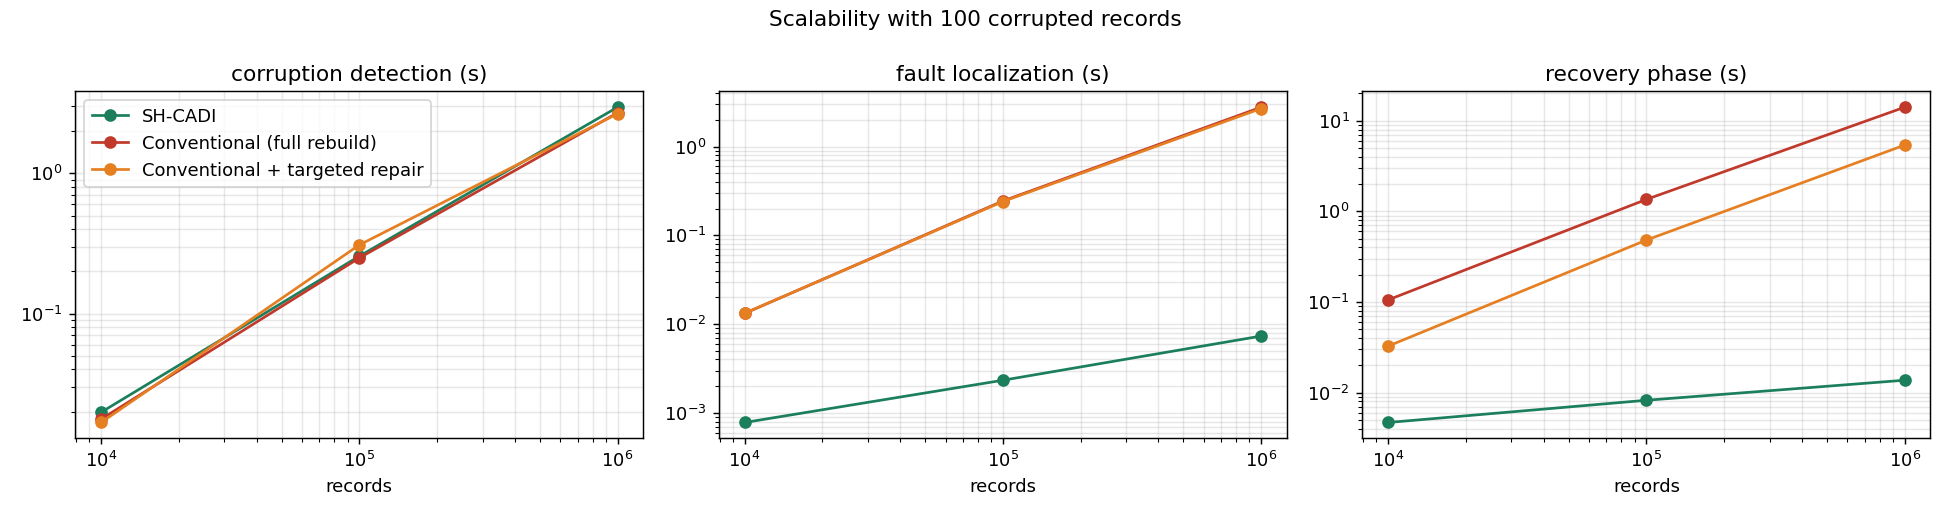
\includegraphics[width=\textwidth]{scalability.png}
\caption{Detection, localization and recovery-phase time against index size with 100 corrupted records (log-log axes).}
\label{fig:scale}
\end{figure*}

\begin{figure*}[t]
\centering
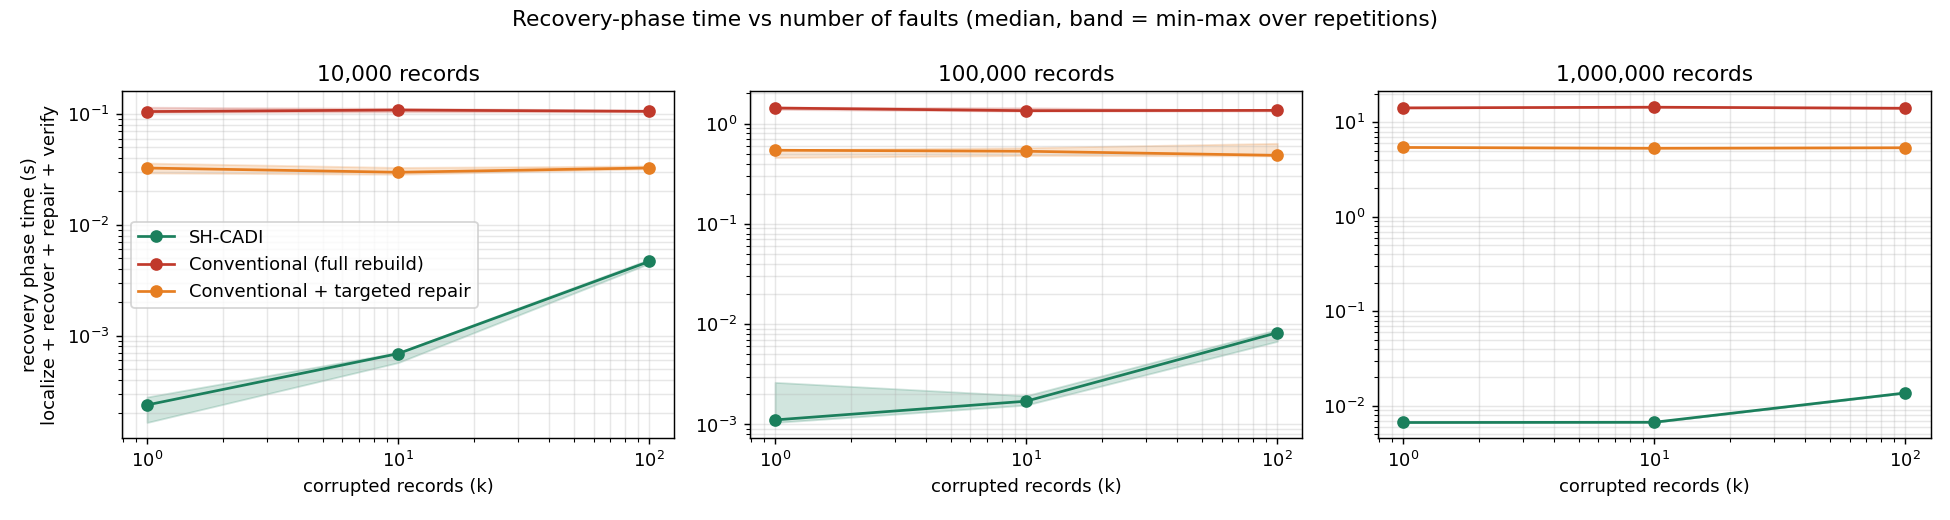
\includegraphics[width=\textwidth]{recovery_vs_faults.png}
\caption{Recovery-phase time against the number of corrupted records for each index size. Bands show the minimum and maximum over repetitions.}
\label{fig:faults}
\end{figure*}

\subsection{Corruption Rate}

The advantage of localized recovery depends on how much of the index is damaged (Table~\ref{tab:rate}, Fig.~\ref{fig:rate}). At 100,000 records, SH-CADI's recovery phase was 72$\times$ faster than targeted repair at 0.1\% corruption but only 1.35$\times$ faster at 25\%, when most buckets are damaged and the descent visits most of the tree. In an earlier run on a single-CPU Linux machine the two were level at 25\%, so we treat that point as approximately equal. The full rebuild stayed near 1.3~s at every rate.

\begin{table}[t]
\centering
\caption{Recovery phase (ms) against corruption rate, 100,000 records}
\label{tab:rate}
\footnotesize
\begin{tabular}{@{}rrrrr@{}}
\toprule
Rate & Faults & Full rebuild & Targeted & SH-CADI \\
\midrule
0.1\% & 100 & 1,357 & 644 & 9.0 \\
1\% & 1,000 & 1,307 & 594 & 57.0 \\
5\% & 5,000 & 1,363 & 687 & 254 \\
10\% & 10,000 & 1,322 & 918 & 472 \\
25\% & 25,000 & 1,330 & 1,280 & 944 \\
\bottomrule
\end{tabular}
\end{table}

\begin{figure}[t]
\centering
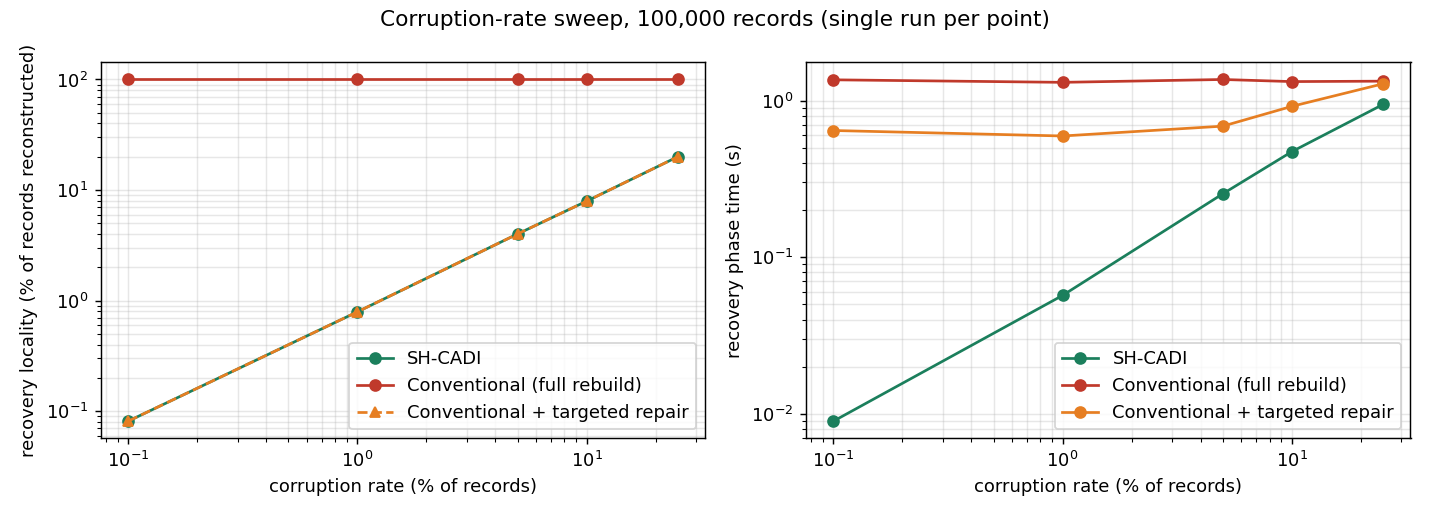
\includegraphics[width=\columnwidth]{rate_sweep.png}
\caption{Recovery locality (left) and recovery-phase time (right) against corruption rate, 100,000 records, one run per point.}
\label{fig:rate}
\end{figure}

\subsection{Robustness to Lost Recovery Information}

We injected 10 metadata faults and also wiped one journal shard that held no faulty record (Table~\ref{tab:shard}). The full rebuild replays the journal for every record, so it lost the healthy records of the wiped shard and failed verification. Targeted repair and SH-CADI lost no records. This robustness comes from repairing only damaged records, not from the Merkle tree itself.

\begin{table}[t]
\centering
\caption{Healthy records lost when one journal shard is wiped}
\label{tab:shard}
\footnotesize
\begin{tabular}{@{}lrrrl@{}}
\toprule
System & 10k & 100k & 1M & Recovered \\
\midrule
Full rebuild & 4 & 2 & 6 & No \\
Targeted repair & 0 & 0 & 0 & Yes \\
SH-CADI & 0 & 0 & 0 & Yes \\
\bottomrule
\end{tabular}
\end{table}

\subsection{Normal-Operation Cost}

Upload throughput was measured on 8,000 chunks of 4~KB with 50\% duplicates. A hash table alone processed 132,729 chunks/s, the hash table with a journal 67,011 chunks/s, and SH-CADI 21,590 chunks/s (88.4~MB/s), because every write verifies and updates a Merkle path. Inserts took 58.0~$\mu$s against 8.6~$\mu$s. At 1,000,000 records, plain lookups (0.98 against 0.59~$\mu$s) and clean full verification (3.44 against 2.76~s) were also slower, while memory after build was 4\% lower (1,281 against 1,336~MB) and the journal was the same size. An authenticated read that finds and repairs a corrupted record took 33, 48 and 55~$\mu$s at 10,000, 100,000 and 1,000,000 records.

%=====================================================================
\section{Discussion and Limitations}
\label{sec:discussion}

SH-CADI's gains are in localization and recovery. Detection still reads every record, so end-to-end improvements (2.7--5.7$\times$ at one million records) are much smaller than recovery-phase improvements. Writes are the main cost.

The results have the following limitations:
\begin{itemize}
\item The implementation is single-threaded pure Python; absolute times would be lower in a compiled language, so ratios are more meaningful than absolute values.
\item The one-million-record results are from a single run and have no variance estimate.
\item The journal is held in memory; disk and network I/O are not modelled.
\item Faults are synthetic and uniformly random; correlated damage is tested only by the wiped-shard scenario.
\item The threat model covers accidental faults with a trusted root; an adversary able to change the root is out of scope.
\item \code{referenced\_by} is not covered by the record digest and is restored on a best-effort basis.
\item There is no concurrency control, and chunking is fixed-size rather than content-defined.
\item The literature check was limited and does not establish novelty.
\end{itemize}

The mid-review proposal also listed a fault-tolerant chunk placement strategy and dynamic redundancy optimization. The first is realized as RS(4,2) with one fragment per node; the second was not implemented, in order to keep the focus on the self-healing index.

%=====================================================================
\section{Conclusion and Future Work}
\label{sec:conclusion}

We designed, implemented and evaluated SH-CADI, a self-healing content-addressable index for deduplicating cloud storage. A chained hash table, a fixed-shape bucketed Merkle tree and a journal sharded with the tree's bucket partition allow the index to detect corruption, localize it to the damaged records, recover only those records, accept them only if they match the authenticated tree, and verify that the trusted root is restored. Chunk data is protected separately with RS(4,2) erasure coding. At one million records with 100 faults, SH-CADI reconstructed 84 records instead of one million and completed its recovery phase 1,030$\times$ faster than a full rebuild, at the cost of slower writes. The advantage shrinks as the corruption rate approaches 25\%.

Future work includes detection without a full $O(n)$ pass (incremental or sampled scrubbing), a disk-backed journal and a compiled implementation, correlated and adversarial fault models, concurrency control, content-defined chunking, dynamic redundancy per chunk, and a systematic literature survey.

The implementation code is available at \url{https://github.com/dkansagara12-alt/SH-CADI}.

%=====================================================================
\begin{thebibliography}{10}

\bibitem{leeseo}
M.~Lee and M.~Seo, ``Secure and efficient deduplication for cloud storage with dynamic ownership management,'' \emph{Applied Sciences}, vol.~13, no.~24, Art. no.~13270, 2023, doi: 10.3390/app132413270.

\bibitem{speeddedup}
P.~Hamandawana, D.-J. Cho, and T.-S. Chung, ``Speed-Dedup: A new deduplication framework for enhanced performance and reduced overhead in scale-out storage,'' \emph{Electronics}, vol.~13, no.~22, Art. no.~4393, 2024, doi: 10.3390/electronics13224393.

\bibitem{mean}
J.~Xia, G.~Cheng, L.~Luo, D.~Guo, P.~Lv, and B.~Sun, ``The doctrine of MEAN: Realizing deduplication storage at unreliable edge,'' \emph{IEEE Trans. Parallel Distrib. Syst.}, 2023, doi: 10.1109/TPDS.2023.3305460.

\bibitem{livededup}
C.-H. Ng, M.~Ma, T.-Y. Wong, P.~P.~C. Lee, and J.~C.~S. Lui, ``Live deduplication storage of virtual machine images in an open-source cloud,'' in \emph{Proc. Middleware 2011}, Lisbon, Portugal, 2011, pp.~81--100, doi: 10.1007/978-3-642-25821-3\_5.

\bibitem{venti}
S.~Quinlan and S.~Dorward, ``Venti: A new approach to archival storage,'' in \emph{Proc. 1st USENIX Conf. File and Storage Technologies (FAST)}, Monterey, CA, USA, 2002.

\bibitem{datadomain}
B.~Zhu, K.~Li, and H.~Patterson, ``Avoiding the disk bottleneck in the Data Domain deduplication file system,'' in \emph{Proc. 6th USENIX Conf. File and Storage Technologies (FAST)}, San Jose, CA, USA, 2008, pp.~269--282.

\bibitem{dynamo}
G.~DeCandia \emph{et al.}, ``Dynamo: Amazon's highly available key-value store,'' in \emph{Proc. 21st ACM Symp. Operating Systems Principles (SOSP)}, Stevenson, WA, USA, 2007, pp.~205--220.

\bibitem{merkle}
R.~C. Merkle, ``A digital signature based on a conventional encryption function,'' in \emph{Advances in Cryptology -- CRYPTO '87}, LNCS, vol.~293. Berlin, Germany: Springer, 1988, pp.~369--378.

\bibitem{reedsolomon}
I.~S. Reed and G.~Solomon, ``Polynomial codes over certain finite fields,'' \emph{J. Soc. Ind. Appl. Math.}, vol.~8, no.~2, pp.~300--304, 1960.

\bibitem{sha}
National Institute of Standards and Technology, ``Secure Hash Standard (SHS),'' FIPS PUB 180-4, Aug. 2015.

\end{thebibliography}

\end{document}
